\documentclass[12pt, a4paper]{article}
\usepackage[brazilian]{babel}
\usepackage{lipsum}
%gera texto aleatorio
\usepackage[utf8]{inputenc}
\usepackage{graphicx}
\usepackage{placeins}
%pacote reconhece acentuação

\title{Projeto de implantação de cabeamento estruturado para uma organização militar}
\author{Raimundo Martins de Araújo Júnior\\Universidade Tecnológica Federal do Paraná}


\begin{document}
	\maketitle
	\begin{abstract}
		Esse trabalho apresenta uma proposta de implantação de cabeamento estruturado para uma organização militar que, atualmente possui uma rede em funcionamento, mas devido a sua escalabilidade o cascateamento da rede fica cada vez mais nítido. Para que a rede tenha uma melhoria é necessário implementar métodos que coíbam tal cascateamento. A ideia é utilizar os procedimentos adotados na NBR e obter um melhoramento nas taxas de transmissão da rede e propor ao mesmo tempo a certificação do cabeamento. 
	\end{abstract}
\vspace{8cm}
\centerline{\textit{\textbf{\today}}}
\newpage
\tableofcontents
\newpage
\listoftables
\listoffigures
\newpage
%\vspace{4cm}
	\section{Introdução}
	O 1º Grupo de Artilharia de Campanha de Selva, sediado em Marabá, estado do Pará possui atualmente uma infra-estrutura de rede com quarenta e dois (42) computadores e dois (2) servidores que auxiliam os serviços administrativos dessa organização militar. Os colaboradores são divididos por seções que formam o organograma que são responsáveis pela execução de suas respectivas atividades.
	\par
	\cite{fourozan10}Além da precisão na entrega, a confiabilidade das redes é medida pela frequência de falhas, pelo tempo que um link leva para se recuperar de uma falha e pela robustez da rede em caso de uma catástrofe.
	\par 
	O objetivo dessa proposta é melhorar o tráfego dos dados que, devido ao crescimento da rede fica cada vez mais cascateado. Futuramente pretende-se expandir a rede para outros prédios, onde ficam os militares da parte operacional da organização.
	\par
	\cite{comer}"As redes de computadores têm crescido explosivamente." \cite{comer} Ainda fala que, "Órgãos governamentais em níveis federal, estadual e municipal utilizam redes, assim como organizações militares."
	\subsection{Benefícios}
	Os benefícios estariam em padronizar a rede conforme a NBR 14565 da ABNT que regula os procedimentos básicos para elaboração de projeto de cabeamento de telecomunicações para rede interna estruturada. Isso faria com que houvesse uma grande melhoria na integridade dos dados, além de colocar a organização em um patamar elevado por se tratar de uma rede que irá seguir as normas.
	\section{Estado atual}
	Atualmente a rede conta com uma infra-estrutura em funcionamento, mas sem a organização necessária para um desempenho de comunicação desejável. A rede foi projetada para a utilização de no máximo quinze (15) computadores, mas com o avanço da tecnologia se faz necessário a aquisição de um número cada vez mais crescente de máquinas, devido ao surgimento de novas funções dentro da organização.
	\par
	Os passivos da rede utilizados no presente momento são:
	\begin{description}
		\item[Path Panel] Atualmente a rede possui apenas um path panel que fica no servidor na seção de informática.
		\item[Cabeamento] O cabeamento utilizado atualmente é o de categoria 5.
		\item[Switch] A rede possui apenas um switch gerenciável, que fica na seção de informática.
		\item[Hub] Existem atualmente seis (6) hubs responsáveis por interligar as seções da organização com o servidor.
	\end{description}
	\par
	Analisando a situação atual da rede, é necessário realizar uma série de mudanças. Uma delas é a atualização dos cabos de categoria 5 para cat6a. Outra mudança relevante é eliminar o uso de hubs pela rede, visto que a sua utilização interfere no desempenho da rede, a solução seria que saísse do switch principal no servidor um cabo para cada computador na rede, e nas seções sejam instalados mutoas (ponto de consolidação) para interligar as máquinas ao servidor, mas levando em consideração a distância máxima do switch até o mutoa e adiante ao terminal do usuário.
	\par 
	Essas mudanças não é algo vago ou aleatório, essa proposta é fruto de estudo com a experiência de usuário em relação ao desempenho atual da transmissão de dados. Há com bastante frequência reclamações sobre falta de internet, conexão lenta, sendo que, é disponibilizado um link de 8 Mb para a intranet do Exército e 1 Mb para sites externos.
	\par 
	Com tais constatações e avaliando a rede física verificamos que a infra-estrutura está ultrapassada e necessita de uma renovação de equipamento, material e também de conceito, assim necessitando do cabeamento estruturado.
	
	\section{Usuários e aplicativos}
	Os usuários atuais fazem parte da administração da organização militar, mas a parte operacional da organização também gera muita documentação de pessoal. Em 2010 foi criado um sistema web de nome SPED, que elimina o uso de papel, ou seja, toda documentação será feita nesse sistema. Assim, se faz necessário uma evolução da rede para os outros prédios existentes, consequentemente o número de usuários ira aumentar.	
	\subsection{Usuários}
	Os usuários são divididos por seções, que são:
	\begin{description}
		\item[1ª Seção] Departamento Pessoal, onde é gerado toda documentação de caráter pessoal dos militares.
		\item[2ª Seção] Departamento de inteligência, onde é avaliado as medidas de contra-inteligência a favor da organização militar, investigações de pessoal interno e externo.
		\item[3ª Seção] Departamento de Operações, onde é feito o planejamento estratégico anual das operações.
		\item[4ª Seção] Departamento de fiscalização administrativa, responsável pela parte de patrimônio e fiscalização dos recursos gastos.
		\item[5ª Seção] Relações públicas, contato com o público externo.
		\item[SALC] Setor de licitações e compras de material permanente ou de expediente.
		\item[Tesouraria] Recebe os recursos e direciona ao setor de licitações.
		\item[Comandante e subcomandante] Respectivamente comandante e subcomandantes, são usuários de nível gerencial mais alto de uma organização militar.
		\item[SECINFO] Usuários analistas e/ou técnicos de informática.
	\end{description}
	
	\subsection{Aplicativos}
	Com o avanço da tecnologia, os sistemas do Exército Brasileiro agora em sua maioria ficam em nuvem, ou seja, não utilizam mais a infra-estrutura da organização para armazenar os sistemas.
	\par 
	Os sistemas utilizados atualmente são:
	\begin{description}
		\item[SPED] Sistema de protocolo eletrônico responsável por tramitar a documentação interna e externa.
		\item[SISCOFIS] Sistema de controle fisico, responsável pelo inventário de todo material carga da organização militar.
		\item[Intranet] Site interno onde ficam armazenado as informações principais, modelos de documentações e etc.
		\item[Sispeg web] Responsável pelo cadastramento de processos internos a organização, o conhecido plano de excelência gerencial.
	\end{description}
	
	\section{Estrutura do prédio principal}
	\par 
	A estrutura do prédio da administração possui um andar e o seu térreo, sendo que, 98\% das seções que funcionam como o coração da organização estão localizadas no térreo do prédio administrativo, possuindo uma grande quantidade de cabeamento horizontal(Horizontal Cabling). É importante mencionar que esse prédio possui em sua estrutura com eletrocalhas, onde a mesma pode ser reaproveitada para a passagem do novo cabeamento, cujo esse projeto propõe.
	\par 
	Os computadores conectados a rede recebem o sinal através de cabeamento par trançado proveniente dos hubs existentes em seções estratégicas. O layout atual da rede obedece a norma que prevê uma distância de no máximo noventa ou cem metros de cabeamento par trançado e do switch para a máquina do usuário de no máximo cinco metros
	\par 
	Ainda sim o tráfego na rede continua com uma lentidão, e as vezes até perca de conexão, reclamação feita por usuários. O prédio administrativo possui dimensões de aproximadamente 50m x 10m. É Considerado um espaço que, se implementar um projeto de cabeamento estruturado a rede tem tudo para ter um bom tráfego. Ainda que a rede seja expandida, como é previsto não atingiria os 100 metros de distância.
	\par 
	A sala de equipamentos (Equipment room) deve ser readequada, a organização da rede deve ser organizada, nada mais justo que começar pela seção de informática onde ficam os servidores, os aplicativos que ainda não foram migrados para as nuvens.
	\section{Planta Lógica}
	\FloatBarrier
	\begin{figure}[!htp]
		\centering
		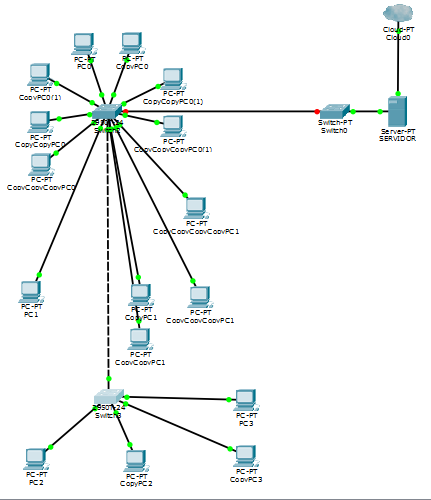
\includegraphics[scale=0.7]{unnamed0.png}
		\caption{Planta lógica da rede}
	\end{figure}
	\FloatBarrier
	\par 
	Na figura acima verificamos a planta lógica da rede, onde podemos constatar as informações descritas anteriormente nessa proposta. A rede está em funcionamento, mas não em 100\% da perfomance desejável. 
	\subsection{Estado atual}
	\FloatBarrier
	\begin{figure}[!htp]
		\centering
		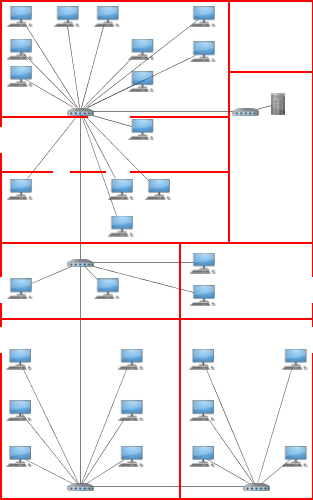
\includegraphics[scale=0.9]{unnamed0.jpg}
		\caption{Estrutura do prédio}
	\end{figure}
	\FloatBarrier
	\FloatBarrier
	\begin{figure}[!htp]
		\centering
		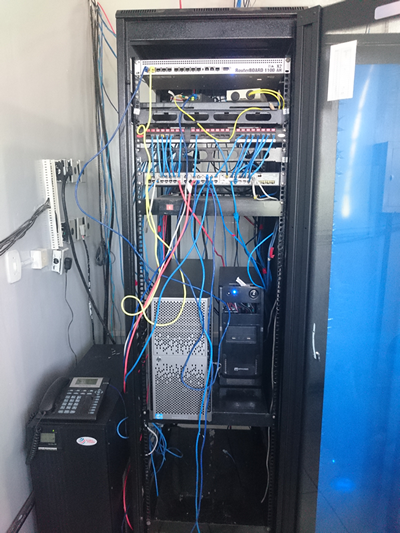
\includegraphics[scale=0.9]{atual_rack.png}
		\caption{Estado atual do rack}
	\end{figure}
	\FloatBarrier
	Como pode ser visto, a situação do rack que fica na seção de informática encontra-se desorganizado, sem identificação dos cabos que chegam, sem um tamanho adequado dos cabos, mas nada diferente do que 60\% dos servidores em organizações pelo país.
	\subsection{Topologia}
	\FloatBarrier
	\begin{figure}[!htp]
		\centering
		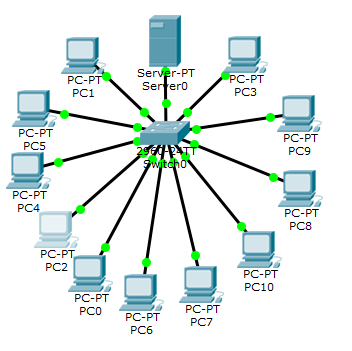
\includegraphics[scale=0.9]{newdiagram.png}
		\caption{Estrutura do prédio}
	\end{figure}
	\FloatBarrier
	Acima vemos a topologia desejável com a implementação do projeto. A mesmo continuaria sendo em forma de estrela, mas da forma como está sendo proposta, eliminaria o uso de hubs pela rede, fazendo a ligação servidor cliente de forma direta, apenas com o intermédio do ponto de consolidação (mutoa), que por sua vez seria instalado nas seções estratégicas.
	\FloatBarrier
	\begin{figure}[!htp]
		\centering
		\includegraphics[scale=0.9]{server.png}
		\caption{Servidor principal}
	\end{figure}
	\FloatBarrier
	Acima podemos observar os componentes  do servidor existente na seção de informática. O mesmo deve receber um patch panel novo visando uma expansão da rede. Logo abaixo podemos verificar a descrição de cada componente.
	\FloatBarrier
	\begin{table}[]
	\centering
	\label{my-label}
	\begin{tabular}{|l|l|}
	\hline
	Componente    & Função                                                                                                                             \\ \hline
	Rack 1        & \begin{tabular}[c]{@{}l@{}}Onde é alocado os servidores, patch panels \\ da seção de informática\end{tabular}                      \\ \hline
	Patch panel 1 & \begin{tabular}[c]{@{}l@{}}É o responsável por receber todos os cabos\\ da rede.\end{tabular}                                      \\ \hline
	Servidor 1    & Servidor de arquivos utilizando o samba4.                                                                                          \\ \hline
	Servidor 2    & \begin{tabular}[c]{@{}l@{}}Servidor virtualização. Existe atualmente os\\ serviços de: DCHP, FTP, Servidor web, SPED.\end{tabular} \\ \hline
	\end{tabular}
	\caption{Descrição de componentes do servidor}
\end{table}
	\FloatBarrier
	
	\FloatBarrier
	\begin{figure}[!htp]
		\centering
		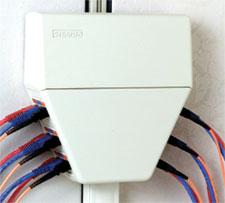
\includegraphics[scale=0.9]{mutoa.jpg}
		\caption{Equipamento mutoa}
	\end{figure}
	\FloatBarrier
	MUTOA é um sistema de cabeamento estruturado para cabeamento horizontal que recebe os cabos e se torna uma espécie de ponto de consolidação, um equipamento que diferentemente do hub não vai prejudicar no tráfego da rede, pois apenas serve como uma ponte entre o servidor e o usuário final.
	\par 
	Abaixo podemos ver como ficaria o funcionamento de um mutoa na organização militar onde é proposto esse projeto:
	\FloatBarrier
	\begin{figure}[!htp]
		\centering
		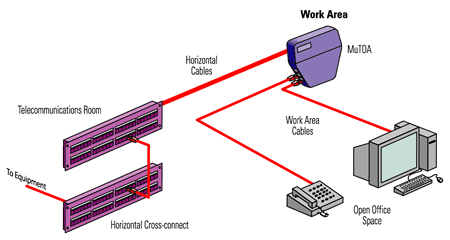
\includegraphics[scale=0.9]{mutoa2.png}
		\caption{Equipamento mutoa}
	\end{figure}
	\FloatBarrier
	
	\subsection{Encaminhamento}
	Atualmente já existe uma estrutura com eletrocalhas no prédio administrativo para alocar a quantidade de cabos utp necessários para interligação servidor-cliente. A mesma pode ser aproveitada, porém, visando a expansão da rede é necessário adquirir uma grande quantidade já visando a escalabilidade dos serviços.
	A estrutura com eletrocalhas possui quatro anos e se encontra em perfeito estado. A mesma irá contribuir na futura execução do projeto. Podemos ver na figura abaixo a eletrocalha chegando no rack.
	\FloatBarrier
	\begin{figure}[!htp]
		\centering
		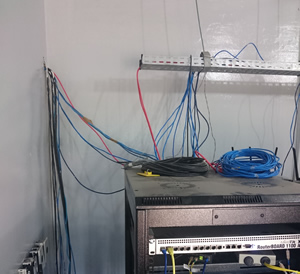
\includegraphics[scale=0.9]{eletr.jpg}
		\caption{Eletrocalha chegando ao rack}
	\end{figure}
	\FloatBarrier
	\subsection{Inventário de passivos}
	Nessa seção serão apresentados os equipamentos e materiais necessários para a implementação do projeto proposto nesse documento.
	\subsubsection{Seção de informática}
	\FloatBarrier
	\begin{table}[]
		\centering
		\label{my-label}
		\begin{tabular}{|c|c|c|c|}
			\multicolumn{1}{c}{\textbf{Produto}}                              & \textbf{Tipo} & \textbf{Fabricante} & \textbf{Quantidade} \\
			\begin{tabular}[c]{@{}l@{}}Patch panel\\ (48 portas)\end{tabular} & CAT-PN-P48Q6  & Pacific             & 2                   \\
			Punch down                                                        & Punch down    & Furukawa            & 2                   \\
			\begin{tabular}[c]{@{}l@{}}Rotulador\end{tabular}    & Eletrônico    & Brother             & 1                  
		\end{tabular}
		\caption{Equipamentos para a seção de informática}
	\end{table}\textsl{}
	\FloatBarrier
	\subsubsection{Complementar da rede}
	\FloatBarrier
	\begin{table}[]
	\centering
	\label{my-label}
	\begin{tabular}{lllc}
		\textbf{Produto}                                         & \textbf{Tipo}                                                              & \textbf{Fabricate} & \multicolumn{1}{l}{\textbf{Quantidade}}                           \\
		Cabo UTP                                                 & Cat 6e                                                                     & Furukawa           & 2 caixas (305m)                                                   \\
		MUTOA                                                    & \begin{tabular}[c]{@{}l@{}}Modular\\ 12 portas\end{tabular}                & Furukawa           & 5                                                                 \\
		Conector                                                 & RJ-45                                                                      & Multilaser         & \begin{tabular}[c]{@{}c@{}}1 Pacote\\ (100 unidades)\end{tabular} \\
		\begin{tabular}[c]{@{}l@{}}Conector\\ Fêmea\end{tabular} & \multicolumn{1}{c}{\begin{tabular}[c]{@{}c@{}}Cat 6\\ Branco\end{tabular}} & Multilaser         & \begin{tabular}[c]{@{}c@{}}1 Pacote\\ (100 unidades)\end{tabular}
	\end{tabular}
	\caption{Equipamentos necessário para implementação}
\end{table}

	\FloatBarrier
	\subsection{Identificação dos cabos}
	A identificação dos cabos se dará através da ferramenta de rotulamento eletrônico a ser adquirida e as nomenclaturas serão distribuídas conforme a seção e a máquina do usuário.
	\par 
	Abaixo segue uma lista referente a como serão feitas as  identificações do cabeamento da rede:
	\FloatBarrier
	\begin{figure}[!htp]
		\centering
		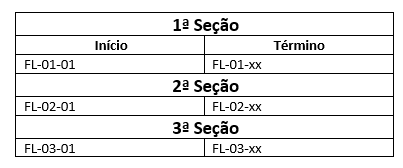
\includegraphics[scale=0.9]{ident.png}
		\caption{Identificação dos cabos}
	\end{figure}
	\FloatBarrier
	
	\section{Cronograma de implantação}
	O projeto caso aprovado iniciará em janeiro de 2017 e seu término é previsto para abril do mesmo ano. O projeto foi analisado e a equipe chefiada pelo 3º Sargento Guarizi descreveu os processos inerentes ao cronograma e através desses dados construímos um gráfico para verificação do tempo de execução de cada atividade. O cronograma foi delineado no famoso gráfico de Gantt, como podemos visualizar na figura a seguir.
	\FloatBarrier
	\begin{figure}[!htp]
		\centering
		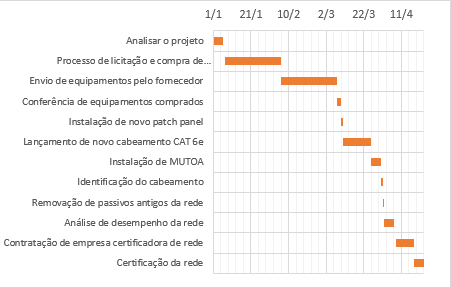
\includegraphics{gantt.png}
		\caption{Cronograma com Gráfico de Gantt}
	\end{figure}
	\FloatBarrier
	\section{Plano de certificação}
	O plano de certificação está incluído no cronograma do projeto e dedica quinze dias para realização da certificação, análise e testes da infra-estrutura de rede.
	\par 
	O processo de certificação é a atividade que vai dar respaldo ao projeto de cabeamento estruturado, mostrando através das analises a melhoria do tráfego de dados na organização.
	
	\section{Plano de manutenção}
	O plano de manutenção não foi incluído no cronograma do projeto, visto que, se a rede após o processo de certificação receber a aprovação, esperasse uma garantia de pelo menos um ano de funcionamento do serviço.
	\par 
	O plano de manutenção se dará no período de seis em seis meses. Se dividirá em dois tipos:
	\begin{description}
		\item[TIPO 1] - Realização de teste na rede através de script de verificação do desempenho do tráfego.
		\item[TIPO 2] - Realização de contato com a empresa certificadora de rede para avaliação da rede. (Obs. Essa ação será realizada somente se os testes do TIPO 1 acusarem mal desempenho da rede)
	\end{description}
	\subsection{Plano de expansão}
	O plano de expansão tem como principal foco inserir os prédios da parte operacional na rede da organização, visto que atualmente os militares tem que se deslocar das companhias para as seções administrativas para confeccionar os documentos do sistema de protocolo eletrônico.
	\par 
	O plano de expansão é um projeto a curto e médio prazo, devendo ser colocado em prática após o processo de certificação da rede, ou seja, quando a rede estiver consolidada através da certificação, executasse a ativadade de expansão da mesma.
	\par 
	Para o plano de expansão deverá se adquirido alguns materiais, o mesmo deve ser adquirido posteriormente a execução do projeto de cabeamento estruturado, visto que, ao comprar o material e deixar guardado com o tempo pode apresentar defeito.
	\FloatBarrier
	\begin{table}[]
	\centering
	\label{my-label}
	\begin{tabular}{|c|c|}
	\textbf{Equipamento} & \textbf{Quantidade} \\
	MUTOA                & 2                   \\
	Computador           & 8                   \\
	Roteador             & 1                  
	\end{tabular}
	\caption{Necessidade de material}
\end{table}
	\FloatBarrier	
	Podemos observar na tabela 3, que adicionamos um roteador. O mesmo se faz necessário visto que uma das salas do prédio operacional ficam os oficiais subalternos (tenentes) e os mesmos não utilizam computadores da organização, utilizam notebooks pessoais. Daí a necessidade de um roteador para que os mesmos possam utilizar a rede do quartel.
	\section{Orçamento}
	Não se pode executar um projeto sem que se saiba os custos do mesmo. É necessário realizar um levantamento de custos de material e também referente a certificação, após isso analisar a viabilidade de recursos para ser alocado nesse projeto.
	\par 
	Fizemos uma lista dos produtos necessários para realização do projeto inicial que visa implementar um processo de cabeamento estruturado na rede e também da aquisição de material para execução do plano de expansão.
	\FloatBarrier
	\begin{table}[]
	\centering
	\label{my-label}
	\begin{tabular}{|l|l|c|l|l|}
		Equipamento                                                                                                                                 & Marca                                                        & \multicolumn{1}{l}{Quantidade}                                     & Preço unitário & Preço total  \\
		\begin{tabular}[c]{@{}l@{}}Patch panel\\ CAT-PN-P48Q6\end{tabular}                                                                          & Pacific                                                      & 1                                                                  & R\$ 295,90     & R\$ 295,90   \\
		Punch down                                                                                                                                  & Furukawa                                                     & 2                                                                  & R\$ 299,98     & R\$ 599,96   \\
		Rotulador eletrônico                                                                                                                        & Brother                                                      & 1                                                                  & R\$ 149,46     & R\$ 149,46   \\
		Caixa De Cabo Utp Cat 6a                                                                                                                     & Furukawa                                                     & 2                                                                  & R\$ 1.107,90   & R\$ 2.215,80 \\
		MUTOA 12 portas                                                                                                                             & Furukawa                                                     & 8                                                                  & x              & x            \\
		Conector RJ-45                                                                                                                              & Multilaser                                                   & \begin{tabular}[c]{@{}c@{}}1 pacote\\ (100 unidades)\end{tabular}  & R\$ 81,00      & R\$ 81,00    \\
		Conector RJ-45 (Fêmea)                                                                                                                      & Keystone                                                     & \begin{tabular}[c]{@{}c@{}}10 pacotes\\ (10 unidades)\end{tabular} & R\$ 69,99      & R\$ 699,99   \\
		\begin{tabular}[c]{@{}l@{}}Computador Intel \\ Dualcore 2gb \\ Hd 320gb Hdmi e \\ Monitor Led 15,6 \\ Triumph Business Desktop\end{tabular} & \begin{tabular}[c]{@{}l@{}}3green \\ Technology\end{tabular} & 8                                                                  & R\$ 949,05     & R\$ 7592,40  \\
		\begin{tabular}[c]{@{}l@{}}Roteador e Repetidor D-link \\ Dir-809 \\ AC 750Mbps Dual-band \\ com 3 Antenas Externas \\ 5dbi\end{tabular}    & D-link                                                       & 1                                                                  & R\$ 137,74     & R\$ 137,74   \\
		Certificação da rede                                                                                                                        & Microlan                                                     & \begin{tabular}[c]{@{}c@{}}42 Pontos de\\ rede\end{tabular}        & R\$ 35,00      & R\$1.470,00 
	\end{tabular}
	\caption{Orçamento de equipamentos}
\end{table}
	\FloatBarrier
	\section{Referências bibliográficas}
	\bibliographystyle{abnTeX2}
	\bibliography{referencia}
\end{document}